\documentclass{beamer}

\usetheme{Warsaw}
%% \usetheme{EastLansing}
%% \usecolortheme{beetle}

\title[Functional Programming]{An Introduction to Functional Programming}
\author{Andreas Pauley -- @apauley}
\institute{Pattern Matched Technologies\\Lambda Luminaries}
\date{September 2, 2013}

\usepackage[utf8]{inputenc}
\usepackage{graphicx}
\usepackage{listings}

\usepackage{hyperref}

\AtBeginSection[]
{
  \begin{frame}
    \frametitle{Table of Contents}
    \tableofcontents[currentsection]
  \end{frame}
}

\begin{document}

\begin{frame}
  \titlepage
\end{frame}

\begin{frame}{Pattern Matched Technologies}
  
\includegraphics[scale=0.21]{img/pmt-logo.png}

  Developing financial applications in Erlang.

  \url{http://www.patternmatched.com/}
\end{frame}

\begin{frame}{Lambda Luminaries}
  \framesubtitle{Local functional programming user group}
  We meet once a month, on the second Monday of the month.

  \url{http://www.meetup.com/lambda-luminaries/}
  
\includegraphics[scale=0.3]{img/LambdaLuminariesScreenShot2013-08-09.png}
\end{frame}

\section{Introduction}

\begin{frame}{A word from the wise}
  \begin{exampleblock}{}
    {\Large ``
      No matter what language you work in, programming
      in a functional style provides benefits.
      You should do it whenever it is convenient, and you
      should think hard about the decision when it isn’t convenient.
      ''}
    \vskip5mm
    \hspace*\fill{\small--- John Carmack, ID Software \cite{carmack}}
  \end{exampleblock}
\end{frame}

\begin{frame}{Quake}
  
\includegraphics[scale=0.4]{img/quake.png}
\end{frame}

\section{Definition of Functional Programming (attempt \#1)}

\begin{frame}{}
  So what exactly is Functional Programming?
\end{frame}

\begin{frame}{Functional Programming (noun):}

  \begin{exampleblock}{}
    {\Huge ``
      Functional Programming is a list of things you CAN’T do.
      ''}
    \vskip5mm
  \end{exampleblock}
\end{frame}

\begin{frame}
  When programming in a functional style/language:
  \begin{itemize}[<+->]
  \item You can't vary your variables.
  \item You can't mutate or change your state.
  \item No while/for loops, sorry.
  \item You can't have side-effects.
  \item You can't control the order of execution (lazy evaluated languages).
  \end{itemize}
\end{frame}

\begin{frame}{Are you kidding me?}
  How can anyone program like this???
  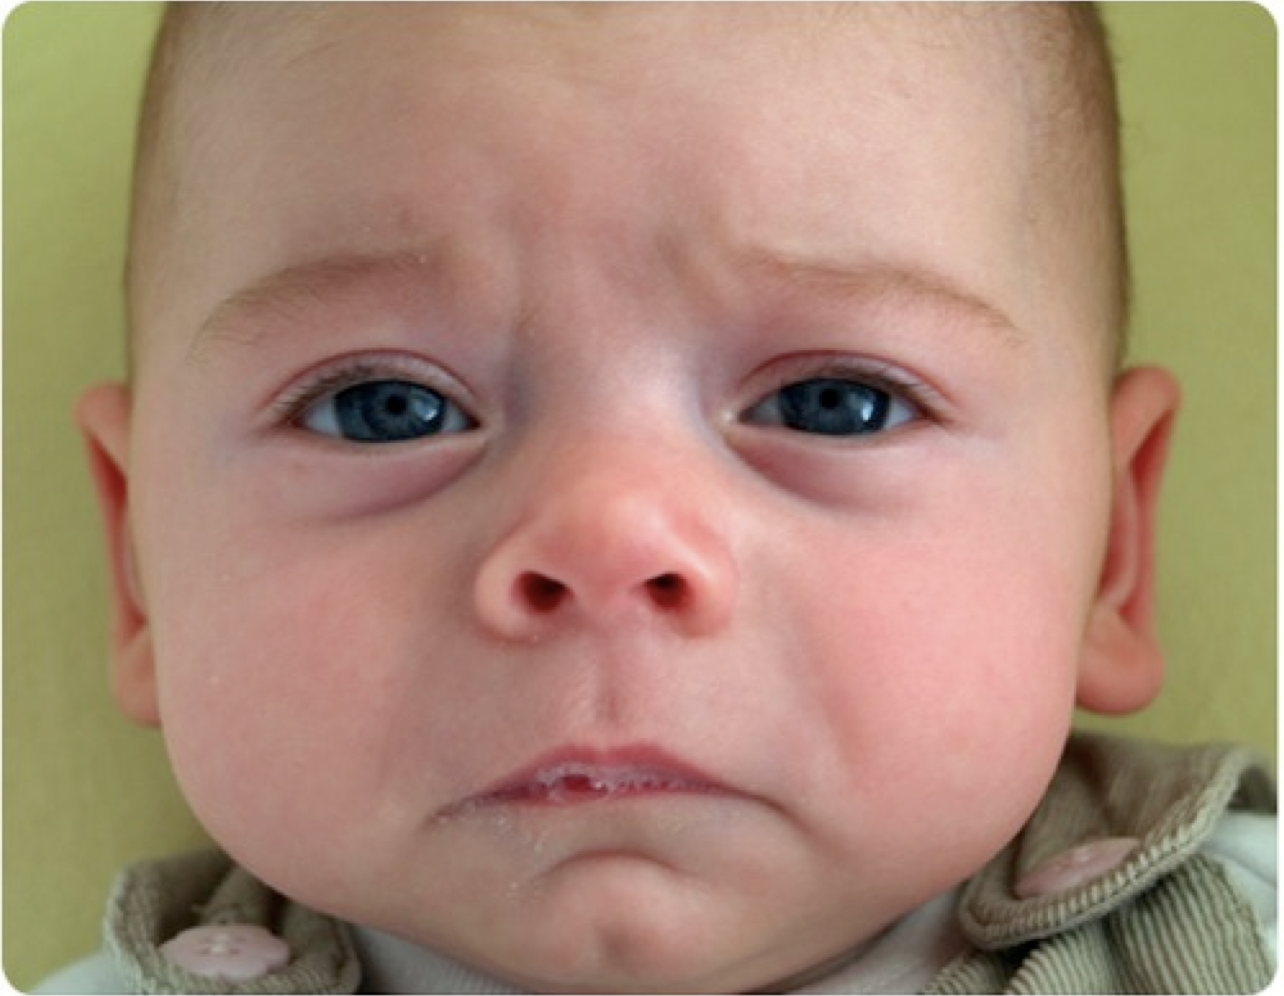
\includegraphics[scale=0.3]{img/sadbaby.png}
\end{frame}

\begin{frame}{GOTO 10}
    This sounds like
  \begin{exampleblock}{}
    {\Large ``You can't have GOTO statements''}
  \end{exampleblock}
  \vskip5mm
  \hspace*\fill{\small See Hughes and Dijkstra \cite{whyfp, dijkstra}}

  \begin{itemize}[<+->]
  \item Also framed in the negative (you can't).
  \item In hindsight we don't really need GOTO's.
  \item In hindsight it is not about what you cannot do.
  \item Benefits of structured procedures with fixed entry/exit points
    has to do with modularity/abstractions etc.
  \end{itemize}
\end{frame}

\begin{frame}{}
  {\Large We need a better definition for Functional Programming.}
\end{frame}

\section{Definition of Functional Programming (attempt \#2)}

\begin{frame}{Functional Programming (noun):}

\begin{exampleblock}{}
  {\Large ``
  Functional programming is so called because a program consists entirely of functions.
  ''}
  \vskip5mm
  \hspace*\fill{\small--- John Hughes, Why Functional Programming
    Matters \cite[p.~1]{whyfp}}
\end{exampleblock}
\end{frame}

\subsection{Function recap}
\begin{frame}{}
OK... so what exactly is a function?
\end{frame}

\begin{frame}{An example function}

  {\Huge $f(x) = 2x + 3$}

\end{frame}

\begin{frame}{Variables in functions}

  {\Huge $f(x) = 2x + 3$}

When we evaluate the function:
  \begin{itemize}[<+->]
    \item $f(4) = 2*4 + 3 = 11$
    \item The value of $x$ will not change inside the function body.
    \item No $x = 4$ and later $x = 21$ in the same function body.
    \item Same input, same output. Every time.
    \item In other words, we can replace any occurrence of $f(4)$ with
      $11$ (Referential Transparency)
  \end{itemize}
\end{frame}


\begin{frame}{Functions can call other functions}

  \begin{itemize}[<+->]
  \item {\Huge $g(x) = f(x) + 1$}
  \item {\Huge $f(x) = 2x + 3$}
  \item {\Huge $g(x) = (2x + 3) + 1$}
  \item {\Huge $g(x) = 2x + 4$}
  \end{itemize}

\end{frame}

\begin{frame}{Values are functions}

  {\large Constant values are just functions with no input parameters}
  \\
  {\Huge $k = 42$}

\end{frame}

\begin{frame}{Functions can be combined}

  \begin{itemize}[<+->]
  \item {\Huge $h(x) = f(g(x))$}
  \item {\Huge $h(5) = f(2(5) + 4)$}
  \item {\Huge $h(5) = f(14)$}
  \item {\Huge $h(5) = 2(14) + 3$}
  \item {\Huge $h(5) = 31$}
  \end{itemize}

\end{frame}

\begin{frame}{Higher-order Functions}

  {\Large Functions can take functions as input and/or return
    functions as the result.}

  \begin{itemize}[<+->]
  \item {\Huge $h(p, q, x) = p(x) + q(2)$}
  \item {\Huge $h(f, g, 3) = f(3) + g(2)$}
  %% \item {\Huge $h(f, g, x) = (2x + 3) + (2(2) + 4)$}
  %% \item {\Huge $h(f, g, x) = (2x + 3) + 8$}
  %% \item {\Huge $h(f, g, x) = 2x + 11$}
  \end{itemize}

\end{frame}

\begin{frame}{Functional Programming (noun):}

  \begin{exampleblock}{}
    {\Large ``
      Functional programming is so called because a program consists entirely of functions.
      ''}
    \vskip5mm
    \hspace*\fill{\small--- John Hughes, Why Functional Programming
      Matters \cite[p.~1]{whyfp}}
  \end{exampleblock}

  \lstinputlisting[language=Python, firstline=3, lastline=8]{code/justfunctions.py}
\end{frame}

%% References
\begin{frame}[allowframebreaks]
  \begin{thebibliography}{10}
    \bibitem{whyfp}
      John Hughes
      \newblock Why Functional Programming Matters
      \newblock \url{http://www.cs.kent.ac.uk/people/staff/dat/miranda/whyfp90.pdf}
    \bibitem{carmack}
      John Carmack
      \newblock Functional Programming in C++
      \newblock \url{http://www.altdevblogaday.com/2012/04/26/functional-programming-in-c/}
    \bibitem{dijkstra}
      Edsger W. Dijkstra
      \newblock Go To Statement Considered Harmful
      \newblock \url{http://www.u.arizona.edu/~rubinson/copyright_violations/Go_To_Considered_Harmful.html}
  \end{thebibliography}
\end{frame}

\end{document}
